%% ==============================
\chapter{\iflanguage{ngerman}{Design}{Concept}}
\label{sec:concept}
%% ==============================


\todo{Formulierung}
Nachdem im vorherigen Kapitel die Methode der Implementierung vorgestellt wurde, beschäftigt sich dieses mit dem Softwaredesign der Implementierung dieser.
\newline
Die Implementierung dieser Bachelorarbeit teilt sich dabei in zwei verschieden Programme auf. Zum einen den sogenannten \textit{VolumeRenderHelper}, der für das Laden, Umwandeln, Verarbeiten und Speichern der Volumendaten zuständig ist. Zum anderen das Unityprogramm \textit{VolumeRenderer}, welches zur Visualisierung der vom Helper erzeugten Daten dient. Diese beiden Programme existierten bereits vor dieser Arbeit und sind in Vorarbeiten des IPRs entstanden. In dieser Bachelorarbeit wurde der \textit{VolumeRenderHelper} um die vorgestellte Transferfunktion erweitert und der \textit{VolumeRenderer} geringfügig angepasst. Die Beiden Programme werden im folgenden als Helper und Renderer erwähnt. Weiterhin wurde ein Pythonskript \textit{PlotHelper} geschrieben, um LH-Histogramme anzuzeigen.
\newline
\todo{christians paper}
\todo{unity und stefffens zeug genauer erklären}
\todo{csharp erwähnen und allgemeine umgebung}
Anfangs liegen die CT-Daten von den Volumen in mehreren Dateien als Schnittbilder im DICOM Format vor. Diese werden mithilfe der MITK Workbench zu einer einzelnen Datei im .nrrd Format umgewandelt, da nur Volumen in diesem Format vom Helper eingelesen werden können.
\newline
Die interne Speicherung des Volumens wird mit der generischen Klasse \textit{Volume} umgesetzt. Diese besitzt ein dreidimensionalen Array vom angegebenen generischen Datentyp, sowie Informationen über das Volumen, wie zum Beispiel Größe der Voxel oder Anzahl der Elemente pro Achse. Des Weiteren bietet die Klasse verschieden Funktionen um Informationen auszulesen oder zu bearbeiten. Zur Darstellung von dreidimensionale Koordinaten, werden die Klassen \textit{IVector3} und \textit{FVector3} benutzt. Diese stellen Vektoren dar, die entweder Integer, Ganzzahlen, oder Float, Dezimalzahlen, als $x,y$ und $z$ Werte speichern.
\todo{Volumenklasse  UML}
\newline
\todo{mergecluster oder clustermerge}
Die Interaktion des Benutzers mit dem Helper findet über eine Kommandozeile statt. Hierbei hat der Anwender die Befehle Load, Dump, Resample, Info, Write, LHHistogram, ClusterVolume und MergeCluster zur Auswahl. Jedes Modul hat dabei seine eigene Syntax die mithilfe eines Help Befehls angezeigt werden kann.
\newline
Die Funktionen der Module entsprechen deren Namen. So lädt Load bespielsweise eine .nrrd oder binäre Datei, Dump und Write speichern das geladene Volumen als binäre oder .nrrd Datei ab, Info gibt Informationen über das aktuell geladene Volumen zurück und Resample lässt den Anwender die Größe des Volumens verändern. Ruft man den Dump Befehl mit einem $u$ am Ende auf, so wird das Volumen vor dem Speichern zum Typ $unsigned$ $int$ gecastet. Dies geschieht indem auf alle Werte der Betrag des minimalen Wertes aufaddiert wird. Dadurch verschieben sich die Werte so, dass das Minimum bei null liegt, also nur noch positive Zahlen im Volumen vorhanden sind. Dies ist für die Darstellung im Renderer wichtig, da dieser nur mit positiven Zahlen funktioniert.
\newline
Im Folgenden werden hauptsächlich die Module LHHistogram, ClusterVolume und MergeCluster erläutert, da diese im Laufe dieser Arbeit entstanden sind. LHHistogram berechnet das LH-Histogramm des geladenen Volumens und speichert dieses in einer .csv Datei ab. ClusterVolume kalkuliert ebenfalls die LH-Werte des Volumens, führt jedoch hinterher noch die beiden Clusteringsschritte des Verfahrens aus. Als Ausgabe speichert das Modul eine binäre Datei eines Volumens, in welchem die verschiedenen IDs der Cluster gespeichert sind. Die Idee dahinter wird im laufe diese Kapitels erklärt. Das Modul MergeCluster dient der Verschmelzung der gewünschten IDs mit dem ursprünglichen Volumen. Das Ergebnis dessen, ist eine finale binäre Datei, die im Renderer das Ventrikelsystem visualisiert. Ein Überblick über den gesamten Aufbau und Ablauf der Implementierung ist in  \autoref{fig:ueberblick} zu sehen.

\begin{figure}
\centering 
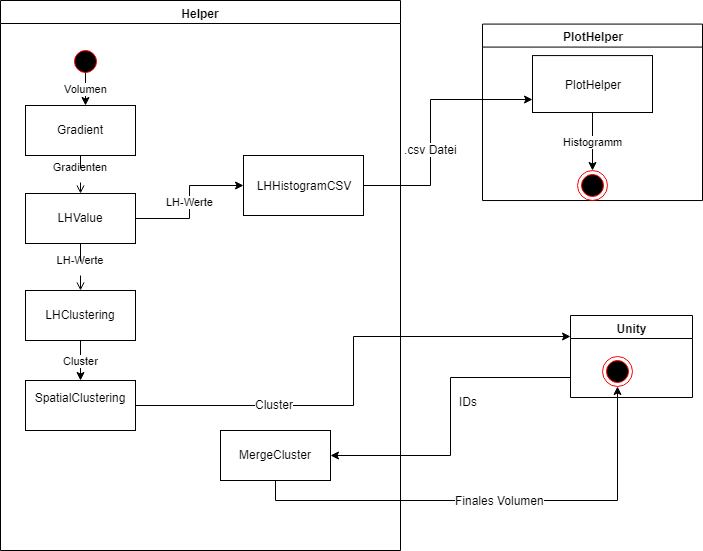
\includegraphics[width=\textwidth]{Logos/Ueberblick.png}
\caption{Überblick über das Programm} 
\label{fig:ueberblick} 
\end{figure}

\todo{abbildung die zeigt warum es das volumen kleiner wird}
\todo{funktionsnamen}
Der Ablauf der Berechnung startet in der statischen \textit{Gradient} Klasse. Diese ist eine Implementierung des Verfahren von Hong \cite{hong2003method}. Zur Berechnung wird der Funktion \textit{bla} das Volumen der Intensitätswerte, als Volumen aus Integern, als Parameter übergeben. Wie im vorherigen Kapitel besprochen, können die Gradienten nicht für einen Voxel direkt berechnet werden, sondern nur für die Punkte zwischen den Voxeln. Aus diesem Grund ist das Ergebnisvolumen um ein Voxel in jeder Achse kleiner als das Volumen der Intensitätswerte, da... (abbildung). Als Ergebnis der Funktion wird ein Volumen vom Typen \textit{FVector3} zurückgegeben.
\newline
DIe Berechnung der LH-Werte findet in der statischen Klasse \textit{LHValues} in der Funktion \textit{LHValueVolume} statt. Als Parameter wird das \textit{FVector3} Volumen der Gradienten aus dem Schritt davor entgegengenommen. Da für die Berechnung der LH-Werte die Intensitätswerte und die Gradienten am gleichen Punkt vorhanden seien müssen, müssen die Intensitätswerte für das verschobene Volumen der Gradienten berechnet werden. Dazu wurde eine einfache Interpolation durchgeführt, indem von allen 8 Nachbarn eines Punktes die Intensitätswerte aufaddiert und hinterher durch acht geteilt wurden. Hierbei muss jedoch beachtet werden, dass die Werte dadurch verändert werden, und Informationen verloren gehen.
\newline
Hat der Benutzer das Modul LHHistogram aufgerufen, wird im Anschluss das LH-Histogramm in der Klasse \textit{LHHistogramCSV} erstellt und wird von ihr als .csv Datei in einem vom Anwender angegebenen Pfad abgespeichert.
\newline
An dieser Stelle kommt das Pythonskript \textit{PlotHelper} zum Einsatz. Dieses lädt die .csv Datei und visualisiert das LH-Histogramm mithilfe einer kalt-zu-heiß-Farbrampe in einem zweidimensionalem Koordinatensystem.
\newline
Hierbei ist zu beachten, dass das Histogramm abhängig von der Häufigkeit des Vorkommens eines LH-Wertpaares im Volumen gebildet wird. Diese werden im jeweils dazu passenden Kästchen des Koordinatensystems gespeichert. Dies ist ein simplerer Vorgehen, als das im Paper von Nguyen \cite{nguyen2012clustering} benutzte Erstellen des Histogramms abhängig von einer für jeden Voxel berechneten Gewichtung. Da die Arbeit an der Implementierung zeitlich beschränkt war, wurde diese Gewichtung, die einzig und allein einer genaueren Darstellung des für das Verfahren irrelevante LH-Histogramm dient, vernachlässigt. Die Gewichtung ist für das Clustering belanglos, da dort ein Histogramm wie oben beschrieben, abhängig von der Häufigkeit der LH-Werte verwendet wird. 
\newline
Wurde jedoch das ClusterVolume Modul aufgerufen, wird mit den beiden Clusteringschritten fortgefahren.
Die Berechnung die in der \textit{LHClustering} Klasse geschieht nimmt das Volumen mit den LH-Werten entgegen und rechnet dieses aus Performancegründen, wie oben beschrieben, in ein ein Histogramm um. Dieser Schritt könnte gespart werden, wenn die Methode \textit{LHValueVolume} direkt ein Histogramm als Rückgabewert liefern würde. Dies würde auch das \textit{LHHistogram} Modul verbessern, da damit die Umrechnung in dieser Klasse ebenso hinfällig wird. Als Ergebnis der Clusteringfunktion \textit{ComputeLHClusters} wird eine Liste der Cluster zurückgegeben, wobei ein Cluster aus einer Liste von \textit{IVector3} besteht. Die Cluster werden nur als Liste der räumliche Informationen der Voxel gespeichert, da für den nächsten Clusteringschritt  lediglich diese Information benötigt wird. 
\newline
Anschließend geht es in der \textit{SpatialClustering} Klasse mit der Berechnung der räumlichen Cluster weiter...
\todo{mehr räumlich clustern beschreiben}
\newline
Nachdem alle Cluster kalkuliert wurden, werden sie in einem Volumen gespeichert. Jeder Cluster bekommt dabei zunächst seine eigene ID beginnend bei eins. Das Volumen wird dann mit den verschiedenen IDs gefüllt. Dies geschieht indem für jeden Cluster an den Positionen der Punkte die jeweilige ID gespeichert wird. Alle anderen Voxel des Clustervolumen wird der Wert null zugewiesen. Dieses Volumen wird als binäre Datei gespeichert und ist das Ergebnis der ClusterVolume Moduls. Es ist bei diesem Modul sehr wichtig, dass es, wie es bei dem Dump Befehl möglich ist, mit einem $u$ am Ende aufgerufen wird, da das Ergebnis sonst nicht vom Renderer dargestellt werden kann.
\newline
Das Ergebnis muss anschließend vom Nutzer in Unity geladen werden. Hierbei kommt die von dieser Arbeit vorgenommenen Anpassung am Renderer zum Einsatz. Dadurch ist es dem Benutzer möglich über ein Eingabefeld während der Visualisierung einen Wert, oder einen Wertebereich anzugeben. Dieser wird dann in einer gewählten Farbe, standardmäßig rot, hervorgehoben. Dies muss der Anwender nutzen, um die IDs, die das Ventrikelsystem beschreiben, zu finden.
\newline
Hat er dies getan kann er mit dem MergeCluster Modul des Helpers das Ergebnis zusammenfügen und die finale Visualisierung erhalten. Beim Aufruf muss der Nutzer das Intensitätsvolumen, das Clustervolumen mit den IDs und die ausgewählten IDs als Parameter übergeben. Anschließend wird an den Stellen der ClusterIDs die Werte im Intensitäsvolumen mit dem Wert 5000 überschrieben, da nach dem beschriebenen Werteshift ins positive der maximale Intensitätswert bei ungefähr 4500 liegt. Dies erhöht das Maximum des Volumens nur gering und lässt es zu die zu visualisierenden Bereiche klar vom Rest abzugrenzen. Dieses Volumen wird erneut als binäre Datei gespeichert.
\newline
Als letzten Schritt kann nun der Benutzer den Wert der eben erklärte Erweiterung des Renderer auf 5000 stellen und die Visualisierung des Ventrikelsystems betrachten.













































